\documentclass[10pt,twocolumn]{article}

%%% PACKAGE SETTINGS %%%
%% Font settings %%
\usepackage[T1]{fontenc}
\usepackage{charter}
\usepackage{algorithm}
\usepackage[noend]{algorithmic}
\usepackage[normalem]{ulem}

%% Custom title page %%
\usepackage[center,small,sc]{titlesec}
\titleformat{\section}{\normalfont\fontsize{13}{13}\bfseries}{\thesection}{.75em}{}
\titleformat{\subsection}{\normalfont\fontsize{12}{12}\bfseries}{\thesubsection}{.5em}{}

%% Custom margins %%
\usepackage[nohead, nomarginpar, margin=.6in, foot=.35in]{geometry}
\setlength{\columnsep}{2em} % set space between two-column format
\setlength{\parskip}{.25em}

%% BibTeX citation pkg
\usepackage{cite}
%% Footnotes

%% Figures, listings with caption %%
\usepackage{hyperref}
\hypersetup{
  colorlinks,
  linkcolor={red!50!black},
  citecolor={blue!50!black},
  urlcolor={blue!80!black}
}
\usepackage{float}
\usepackage{graphicx}
\usepackage[font=normal,labelfont={bf,it},textfont={bf,it}]{caption}

\usepackage{lipsum}
\usepackage{xcolor}
\usepackage{textcomp}
\usepackage{listings}

\lstset{
  basicstyle=\small\ttfamily,
  commentstyle=\ttfamily,
  keywordstyle=\bfseries,
  escapeinside={<@}{@>},
  aboveskip=1pt,
  belowskip=-5pt,
  belowcaptionskip=-3pt,
  frame=single,
  captionpos=b,
  showstringspaces=false,
  columns=flexible,
  linewidth=\columnwidth,
  breaklines=true,
  keepspaces=true,
  identifierstyle=\ttfamily,
  keywordstyle=\ttfamily\color[rgb]{0,0,1},
  commentstyle=\ttfamily\color[rgb]{0.133,0.545,0.133},
  stringstyle=\ttfamily\color[rgb]{0.627,0.126,0.941},
}

%%% DOCUMENT BEGINS %%%
\begin{document}
\author{
        Julien Couvy\\
        Vrije Universiteit Amsterdam\\
        \texttt{julien.couvy@gmail.com}
        \and
        Herbert Bos\\
        Vrije Universiteit Amsterdam\\
        \texttt{herbertb@cs.vu.nl}
        \and
        Cristiano Giuffrida\\
        Vrije Universiteit Amsterdam\\
        \texttt{giuffrida@cs.vu.nl}
}
\title{\Huge Exploiting ROP attacks with a unique instruction\vspace{.75em}}
\maketitle

\begin{abstract}

  \textbf{We present a proof of concept pseudo-compiler that translates a given
    exploit in any language to a return oriented programming payload for a
    target binary. In contrast to other works, we take advantage of the Turing
    completeness of the x86 mov instruction. By only having to handle mov
    instructions instead of the entire ISA, we reduce the complexity of crafting
  payloads while keeping, in theory, the same degree of expressiveness.}

  \textbf{We describe the fundamentals behind ROP attacks, and explain the
    functioning of our tool. In addition, we discuss its limitations and the
    results found using  sample test programs. Finally, we suggest ways to extend
  our work.}

\end{abstract}

\section{INTRODUCTION}

The widespread adoption of \textit{Data Execution Prevention (DEP)}, which
ensures that writable memory regions are non-executable\footnote{also referred
as W$\oplus$X}, such that an attempt to execute machine code in these regions
will cause an exception has largely mitigated classic code injections attacks.
It is deployed in virtually all main operating systems: Linux (first via PaX
patches), OpenBSD, Windows (since XP SP2), OS X (since 10.5), Android and so
on. Hardware now features easy DEP support with an extra flag dedicated to the
marking: Intel "XD" and AMD "NX" to name a few.

DEP techniques largely killed classic code injection attacks.  However, as one
exploit faded another arose. In 1997, Solar Designer presented a new approach
\textit{return-to-libraries}\cite{solar_returnintolib_1997} attacks. Once the
control-flow of a program was comprised, the attacker would use code
(functions) already present in shared libraries. As no code injection was
required, doing so would bypass the defenses we highlighted. A classic target
was \textit{libc}\footnote{return-to-lib attacks are often referred as
return-to-libc for that reason} that contained subroutines for powerful system
calls that would allow arbitrary code execution. Back then, a common perception
was that removing dangerous \textit{syscalls}\footnote{system() allows to
execute any program with the current \textit{privileges}} from standard libraries
would suffice to stop return-to-libc attacks.  Besides, with the arrival of
Intel's new 64bits x86 processors, the subroutines calling convention was
changed to require most arguments of a function to be passed in registers
instead of on the stack. Shared libraries developers also began to restrict or
remove library functions that performed useful actions for attackers. As a
result, return-to-libraries attacks were much harder to craft successfully and
faded away for a time.

At Black Hat USA 08, Roemer et al.\ presented a Turing-complete exploit
language (initially proposed by Shacham\cite{shacham_rop_2007} at CCS in
2007) capable of arbitrary code execution without relying on shared libraries.
\textit{Return Oriented Programming (ROP)}\cite{roemer_return-oriented_2012}
has now become the main technique of choice for nearly all modern exploits of
memory-safety vulnerabilities.

In this paper, we present \textit{Mov2Rop}, an attempt at creating a ROP
pseudo-compiler that translates an exploit of choice into a gadget chain for a
target binary. In its current state, the only supported architecture is Intel
x86. One of our motivations was to make use of Domas' single instruction
compiler \textit{movfuscator}\cite{domas_movfuscator} based on the observation
that mov instructions are Turing complete\cite{dolan_mov_2013}. Using
movfuscator, we only have to find gadget chains for mov instructions greatly
reducing the complexity of our tool while keeping, in theory, the ability to
compile any exploit in to its ROP equivalent.


\section{BACKGROUND}

\subsection{Process Memory Organization}
We will briefly describe the
organization of processes in memory (see \autoref{fig_memorg}) and recap what is the stack.

Processes are divided into three regions or segments: \textit{Text, Data} and
\textit{Stack}.

\begin{figure}[h]
  \centering
  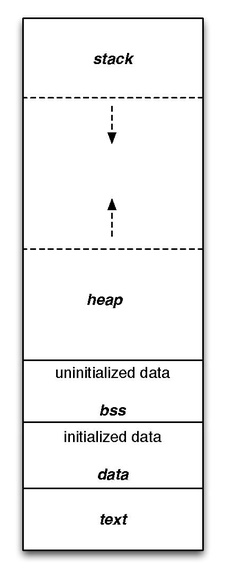
\includegraphics[scale=.85]{./graphics/memory_organization.jpg}
  \caption{Memory organization}
  \label{fig_memorg}
\end{figure}

\textbf{\textit{The text segment,}} also known as code segment, includes the
executable instructions and read-only data. This region corresponds to the text
section of the executable file. It is normally marked read-only and any attempt
to write to it will result in a segmentation violation.

\textbf{\textit{The data segment}} is split in two parts (see
\autoref{lst-variable})
\begin{itemize}
\item Initialized data, simply called data segment
\item Uninitialized data, also known as the bss segment
\end{itemize}
    The data segment contains the global variables and static variables
which have a pre-defined value and can be modified. The BSS segment contains
all global variables and static variables that are initialized to zero or do
not have explicit initialization in source code.

\begin{lstlisting}[aboveskip=\bigskipamount,belowskip=\medskipamount,caption=Variable
<<<<<<< HEAD
location in memory,language=C,label=lst-variable]
=======
location in memory,language=C,label=lst-variable] 
>>>>>>> 8a1659c9aaa397ac58835e3eac58f9366fd16834
// this static variable is stored in the BSS segment
static int bss_variable;
// this global variable is in the DATA segment
int data_variable = 42;
\end{lstlisting}

\textbf{\textit{The heap segment}} is the region where dynamic memory
allocation takes place. The heap area commonly begins at the end of the
\texttt{.bss} and \texttt{.data} segments and grows to larger addresses from
there.

\textit{\textbf{The stack segment,}} a stack is a contiguous block of memory
containing data such as the local variables of functions. It is a \textit{Last In First Out} data structure, which means
literally that the latest value stored on the stack will be the first to be
removed, commonly used
in computers. A register called the \textit{stack pointer} points to
the top of the stack. In addition to the stack pointer, a frame or local base
pointer is also present which points to a fixed location within a frame. Its
size is dynamically adjusted by the kernel at run time.

Every processor \textit{Instruction Set Architecture (ISA)} integrates
instructions to \texttt{push} and \texttt{pop} values onto/off the stack. The
stack consists of logical stack frames that are pushed when calling a function
and popped when returning. In 32bits architectures, a stack frame contains the
parameters to a function, its local variables, and the data necessary to
recover the previous stack frame, including the value of the instruction
pointer at the time of the function call. Depending on its implementation the
stack will grow up or down. In the rest of this paper, we will consider that
the stack grows downwards to reproduce the behavior of Intel processors.

\subsection{Buffer Overflows}

Low level languages directly compiled to machine code such as C/C++ offer wide
possibilities of implementation without the cost of speed. However, this level
of freedom over memory management increases the risk of errors from programmers.
Indeed, many powerful instructions can easily be exploited if used improperly.
Numerous attacks aim at diverting the control-flow during the execution of a
program. Buffer overflows and other memory corruption vulnerabilities still plague many programs and are a main research
topic in computer
security\cite{DBLP:journals/iee/MouzaraniSZ16,DBLP:journals/iee/PadmanabhuniT16,DBLP:conf/ant/LeonB16}.

\lstinputlisting[aboveskip=\medskipamount,belowcaptionskip=0pt,float=h,language=C,firstline=5,label=lst_overflow,caption=Buffer
overflow vulnerability]{./snippets/simple_overflow.c}

A \textit{buffer overflow} attack is an anomaly where a
program, while writing data to a buffer, overruns the buffer's boundary and
overwrites adjacent memory locations. In other words, a buffer overflow condition exists when a program attempts to put more data in a buffer than it can
hold or when a program attempts to put data in a memory area past a
buffer. Overflows can be used to modify return address or code pointers in order
to execute a malicious piece of code, sometimes already existing within the
program's space or injected by the attacker. Buffer overflow vulnerabilities typically occur in code that:
\begin{itemize}
    \item Relies on external data to control its behavior
    \item Depends upon properties of the data that are enforced outside of the immediate scope of the code
    \item Is so complex that a programmer cannot accurately predict its behavior
\end{itemize}

With cautious manipulations, an attacker could grant himself unrestricted
privilege to an unprivileged account or user.

\textbf{\textit{Example:}} \textit{stack-based buffer
overflow}\cite{one_stacksmashing_1996}. When invoking or exiting a standard C
function, the procedure prolog or epilog must be called, this involves saving
the previous variables and allocating space for the new variables; and
vice-versa when the function exits. The previous FP is pushed, a new FP is
created and SP operates with respect to its new local variables.

\textbf{\textit{Procedure:}} in the following program (see
\autoref{lst_overflow}), the
vulnerability comes from a wrong use of \textit{strcpy()}. We disabled ASLR and
Stack Canaries for the sake of simplicity. The target information are the size
of the buffer and the address of \textit{exec\_shell()}. The former will help
us overflow the buffer without going too far which would lead to a segmentation
fault while the latter is the address we want to return to. Any disassembler
tool like \textit{gdb} (see \autoref{lst-gdb}) can give us the information we need to perform the
overflow and spawn a shell (see \autoref{lst-shell}).

\begin{lstlisting}[aboveskip=\bigskipamount,belowskip=\medskipamount,caption=Gdb
output on simple\_overflow.c,label=lst-gdb]
$ gdb -q simple_overflow
(...)
(gdb) disas vuln_func
Dump of assembler code for function vuln_func:
   0x08048524 <+0>:	push   %ebp
   0x08048525 <+1>:	mov    %esp,%ebp
   0x08048527 <+3>:	sub    $0x78,%esp
   0x0804852a <+6>:	sub    $0x8,%esp
   0x0804852d <+9>:	pushl  0x8(%ebp)
   0x08048530 <+12>:	lea    -0x6c(%ebp),%eax
   0x08048533 <+15>:	push   %eax
   0x08048534 <+16>:	call   0x80483a0 <strcpy@plt>
   0x08048539 <+21>:	add    $0x10,%esp
(...)
(gdb) print exec_shell
$1 = (...) 0x80484fb <exec_shell>
\end{lstlisting}

To overwrite the return address with the one of \textit{exec\_shell()} we need
to fill the buffer with $100$ bytes, overwrite SFP\footnote{the saved frame
pointer (old content of \%ebp) is called SFP} with a dummy value and then the
target address. \autoref{lst-stackstate} shows the state of the stack before and
after the overflow.

\begin{lstlisting}[float=h,aboveskip=\bigskipamount,belowskip=\medskipamount,caption=Stack
before and after overflow,label=lst-stackstate]
| <argument>                 |
| <return address>           |
| <old %ebp>                 | <= %ebp
| <0x6c bytes of             |
|       ...                  |
|       buffer>              |
| <argument>                 |
| <address of buffer>        | <= %esp
           BEFORE

| 0x80484fb <exec_shell()>   |
| 0x42424242 <fake old %ebp> | "BBBB" in hex
| 0x41414141 ...             | "AAAA" in hex
|   ... (0x6c bytes of 'A's) |
|   ... 0x41414141           |
           AFTER
\end{lstlisting}

In practice, once the return address is overwritten, the attacker can perform
his exploit via a \textit{code injection} assuming no defenses are in place,
\textit{return-to-libraries} attack, or \textit{return oriented programming}
attack. In the remainder of this paper, we will assume that we deal with a
32bits architecture.

\begin{lstlisting}[float=ht,belowskip=\medskipamount,caption=Spawning a
shell,label=lst-shell]
$ ./simple_overflow "$(python2 -c 'print "A"*0x6c + "BBBB" + "\xfb\x84\x04\x08"')"
Spawning a shell !
sh-4.4$
\end{lstlisting}

\subsection{Return Oriented Programming}
In this section we will introduce the concepts behind \textit{return-oriented programming
}\cite{roemer_return-oriented_2012}.

Return-oriented programming is a technique by which an attacker can induce
arbitrary behavior in a program whose control-flow he has diverted, without
injecting any code. It was built to overcome buffer exploit defense mechanisms
like ASLR (in a non-trivial way), or DEP. The technique consists of aggregating
malicious computation by linking together short code snippets called
\textit{gadgets}.  A \textit{gadget} ends in a \texttt{ret} instruction and is
located in a subroutine within the program's address space. Chained together,
these gadgets allows an attacker who controls the call stack to build and
execute his payload. Because the executed code is stored in memory marked
executable, the W$\oplus$X defense will not prevent it from running.

Return oriented programming can be seen as a generalization of traditional
return-into-lib attacks. But the threat is more general. In theory, ROP can be
used to make Turing complete attacks. However, in practice is quite complex and
very little research exists to automate the creation of Turing complete
exploits.

\textbf{\textit{Example:}} see \autoref{lst_ropchain}. We want to give a
general understanding on how gadget chaining generally works. Here, we need to
concatenate \texttt{"/bin/sh"} in a buffer by chaining functions together and
finally spawn a shell. Each function requires specific parameters that we need
to store on the stack along with the gadget chain. We assume that we have a
memory vulnerability that allows us to perform a stack-buffer overflow in the
same conditions as the last example.

\textbf{\textit{Stack preparation:}} an attacker prepares a fake stack frame to
look like a collection of new return addresses for control-flow changes. In
practice, it is a very meticulous process as we will see in a following
section.

\textbf{\textit{Procedure:}} when the \textit{instruction pointer} points at
the address of \texttt{add\_bin()}, the return address\footnote{see standard C
 function calling procedure} is the address of a
 \texttt{pop; ret;} gadget. The test value is parsed as argument in
 \texttt{add\_bin()}. The \texttt{pop; ret;} gadget ensures that the next value
 pointed by \texttt{\%ip} will be the address of the second gadget in the
 chain. See Appendix \ref{appendix:a} for a written exploit.

\lstinputlisting[aboveskip=\medskipamount,belowcaptionskip=0pt,float=h,language=C,firstline=31,lastline=53,label=lst_ropchain,caption=ROP
exploit example]{./snippets/chaining_func.c}

\begin{lstlisting}[float,aboveskip=\bigskipamount,belowskip=\medskipamount,caption=Stack
prepared with a ROP chain]
| <address of exec_command()> |
| 0xcafebabe <key1>           |
| 0x8badfood <key2>           |
| <address of POP; POP; RET>  |
| <address of add_sh()>       |
| 0xdeadbeef <key>            | <argument>
| <address of POP; RET>       | <return addr>
| <address of add_bin()>      | <function call>
| 0x42424242 <fake old %ebp>  |
| 0x41414141 ...              |
|   ... (0x6c bytes of 'A's)  |
|   ... 0x41414141            | 0x41414141 == "AAAA"
\end{lstlisting}


\section{RELATED WORK}

\textit{Control-flow integrity (CFI)\cite{mulder_subject_2016}} is a property
of a program which says that the flow of execution does not divert from the
intended or original control flow graph. Many techniques were/are being
developed to maintain control-flow integrity. However, recent research also
showed that many of these (dated) defenses can be bypassed.

\textit{Address Space Layout Randomization:} ALSR makes it more difficult for
an attacker to predict the target address. It rearranges the address space
positions of key data areas of a process, including the base of the executable
and the positions of the stack, heap and libraries.

\textit{ShadowStacks:} This technique mitigates return address overwrites by
<<<<<<< HEAD
keeping a record of the legitimate return address for a function call on a
=======
keeping a record of of the legitimate return address for a function call on a
>>>>>>> 8a1659c9aaa397ac58835e3eac58f9366fd16834
separate stack, and then to check that the return address is still correct
before returning.

\textit{Stack Canaries:} They are used to detect a stack buffer overflow before
execution of malicious code can occur. Stack canaries work by modifying every
function's prologue and epilogue regions to place and check a value on the
stack respectively. As such, if a stack buffer is overwritten during a memory
copy operation, the error is noticed before execution returns from the copy
function.

While these techniques improved our defenses against ROP attacks, most of them only
 complexify the infection but do not fix the underlying vulnerability.

\textbf{\textit{ROP Compiler:}} Follner et al.\ presented
PSHAPE\cite{barthe_pshape:_2016}, a state-of-the-art open source gadget
chaining tool adapted to realistic scenarios. It offers syntactic and semantic
gadget search and automatic chaining for 64 bits architectures.  They claim
being the only one amongst competition to successfully create ROP chains
automatically in nine out of eleven practical cases.


\section{MOV2ROP}

In this paper, we are trying to translate a given exploit into a ROP chain for
a target binary. Our work differs from other compilers as we chose to compile
the source code into mov instructions only using an external compiler
\textit{movfuscator}. Mov2Rop is written in Python and is divided into three
different modules: the \textit{Extractor}, \textit{Dissassembler}, and
\textit{Matcher}.

\subsection{Gadget Extraction}

We use Ropper's engine\cite{sashs_ropper} within the Extractor  module to
extract gadgets from binaries. Gadgets are searched according to a regular
expression (see \autoref{lst:ropper}).

\begin{lstlisting}[float=h,aboveskip=\medskipamount,belowskip=0pt,caption=Ropper
search engine,label=lst:ropper]
$ ropper --file target_bin --search "pop e??; ret;"
0x080bbf26: pop eax; ret;
0x08048411: pop ebp; ret;
0x080481d1: pop ebx; ret;
...
\end{lstlisting}

The output is then parsed by our program to create a list of \textit{Gadget}
objects. Gadgets are defined by a list of \textit{Instruction} objects (see
\autoref{lst:instruction}) and the
address of its first instruction. We define an Instruction by a label, an
address, a mnemonic, a source and a destination (without optional offsets).
Mnemonics are short strings representing the type of instruction. A mnemonic is
<<<<<<< HEAD
assigned by looking-up in a dictionary of opcodes (see Table 1). The opcode is extracted
=======
assigned by looking-up in a dictionary of opcodes (see \autoref{tab:opcode}). The opcode is extracted
>>>>>>> 8a1659c9aaa397ac58835e3eac58f9366fd16834
with regular expressions manipulations on Ropper's output.

\begin{lstlisting}[float=h,aboveskip=\medskipamount,belowskip=0pt,caption=Example
instruction object,label=lst:instruction]
Instruction found at <0x80d5386>
---------------------------------
Mnemonic: MOV r32,r/m32
   Label: mov edi, dword ptr [edx]
    Dest: edi
     Src: edx
\end{lstlisting}

\begin{table*}[t]
\centering
\label{tab:opcode}
\begin{tabular}{l|l|l}
\textbf{Opcode} & \textbf{Mnemonic} & \textbf{Description} \\ \hline
0x89 & MOV r/m32,r32 & Memory write (or register move) with 32 bits reg \\ \hline
0x8B & MOV r32,r/m32 & Memory read from 32 bits reg \\ \hline
\begin{tabular}[c]{@{}l@{}}0xB8\\ 0xBB\\ ...\end{tabular} & \multicolumn{1}{c|}{MOV r/m32,imm32} & Memory write from immediate val \\ \hline
\begin{tabular}[c]{@{}l@{}}0xA1\\ 0x8B1D\\ ...\end{tabular} & MOV r32,imm32 & \begin{tabular}[c]{@{}l@{}}Memory read from immediate val\\ ex: mov eax, ds:0x0\end{tabular} \\ \hline
0xA3 & MOV imm32,r32 & Memory write from 32bits reg to imm val \\ \hline
\multicolumn{1}{c|}{...} & \multicolumn{1}{c|}{...} & \multicolumn{1}{c}{...}
\end{tabular}
\caption{Opcode Dictionary}
\end{table*}

\subsection{Payload Treatment}

The source code that we want to translate is firstly compiled to an object file
in Intel syntax using \textit{movfuscator}.  We use
Capstone\cite{quynh_capstone}, a multi architecture disassembly framework to
analyze each instruction. The Disassembler module searches for all \texttt{mov}
instructions and creates Instructions objects similar to Extractor. When
created, an Instruction is assigned a mnemonic reference if the dictionary
lookup was successful, otherwise it's simply referred to as not supported.

\subsection{Instruction Analysis}

The Matcher module will create lists containing each type of gadget. We
divide them in three categories: memory reads, memory writes, and register
moves. The output of the Extractor module is analyzed using an expandable set
of rules (see \autoref{lst:rule}).

\textit{No access on \texttt{esp}}: we rule out any instruction accessing, in
read or write, \texttt{esp}. Because of the nature of ROP, controlling
\texttt{esp} is difficult and it is safer not to use it other than with \texttt{ret}
instructions.

\textit{Restricted instructions:} certain instructions like \texttt{call} or
\texttt{leave} introduce jumps at undetermined addresses.

\textit{Conflict prevention:} gadgets that are not "pure" (i.e: more than one
instruction long, excluding \texttt{ret}) have a chance to contain intermediary
instructions that can disrupt the purpose of the gadget. For example (see
\autoref{lst:rule}), if a
value needs to be stored on a register \texttt{eax} and one intermediary
instruction modifies the content of said register, then the value is lost.
Thus, we rule out any gadget with intermediary instructions that affects the
\texttt{dest} register of the first instruction.


\begin{lstlisting}[float=h,aboveskip=\medskipamount,belowskip=0pt,caption=Rule
verification,label=lst:rule]
X write on ESP
Gadget <0x80a1de3>: g1: mov dword ptr [eax], edx
                    g2: add esp, 8
                    g3: pop ebx
                    g4: ret;

X conflicting instructions
Gadget <0x807af78>: g1: mov eax, dword ptr [eax]
                    g2: sub eax, dword ptr [edx]
                    g3: ret;


\end{lstlisting}

We observed that chains can be found even with these limitations, while fixing
them would require a delicate stack preparation.


\subsection{Gadget Chaining}

The Matcher module is also in charge of chaining gadgets together mapping to
the desired payload instruction.

Firstly, we mapped all possible movements between registers to obtain a general
view. On a very simple program (with glibc statically linked) we got the
following map (see \autoref{lst:map}):

\begin{lstlisting}[float=h,aboveskip=\medskipamount,belowskip=0pt,caption=Map
of movement between registers,label=lst:map]
Possible reg mov:
        src: dst (<> = direct, [] = chained)
        eax: <edi edx> [eax esi ebx ecx] <@\sout{ebp esp}@>
        ebx: <eax> [edi edx esi ebx ecx] <@\sout{ebp esp}@>
        ebx: <eax> [edi edx esi ebx ecx] <@\sout{ebp esp}@>
        ecx: <eax> [edi edx esi ebx ecx] <@\sout{ebp esp}@>
        edx: <eax esi ebx ecx> [edi edx] <@\sout{ebp esp}@>
        ebp: <eax> [edi edx esi ebx ecx] <@\sout{ebp esp}@>
        edi: <eax edx> [esi ebx edi ecx] <@\sout{ebp esp}@>
        esi: <eax esi> [edi edx ebx ecx] <@\sout{ebp esp}@>
\end{lstlisting}

For example on the first line, the map highlights that at least one gadget that
allows to move the content of \texttt{edi} to \texttt{eax}
directly\footnote{with a "pure" gadget constituted of one instruction followed
by a \texttt{ret}}. The map is useful when we need to weave gadgets together
in order to fit a target instruction.

\begin{algorithm}
    \caption{IsMovable(src, dst, register\_move[])}
    \label{alg:is_movable}
<<<<<<< HEAD
    \begin{algorithmic}[1]
=======
    \begin{algorithmic}[1] 
>>>>>>> 8a1659c9aaa397ac58835e3eac58f9366fd16834
        \REQUIRE $register\_move[]$ (gadgets moving regA to regB)

        \FOR{$register$ accessible from $src$}
            \IF{$register \neq src$ $\AND$ $register = dst$}
                \FOR{$gadget$ in $register\_move[]$}
                    \IF{$gadget\_src = src$ \AND $gadget\_dst = register$}
                        \IF{$\NOT\ SearchForConflict()$}
                        \RETURN \TRUE
                        \ENDIF
                    \ENDIF
                \ENDFOR
            \ENDIF
        \ENDFOR

        \FOR{$register$ accessible from $src$}
            \IF{$register\ \NOT$ visited $\AND\ register \neq src$}
                \STATE $register \leftarrow visited$
                \FOR{$gadget$ in $register\_move[]$}
                    \IF{$gadget\_src = src$ \AND $gadget\_dst = register$}
                        \IF{$\NOT\ SearchForConflict()$}
                        \RETURN $IsMovable(register, dst, register\_move[])$
                        \ENDIF
                    \ENDIF
                \ENDFOR
            \ENDIF
        \ENDFOR
        \RETURN $\FALSE$

    \end{algorithmic}
\end{algorithm}

<<<<<<< HEAD
We ensure that no side-effects occur within the gadget chain (see Algorithm
=======
We ensure that no side-effects occur within the gadget chain (see Algorithm 
>>>>>>> 8a1659c9aaa397ac58835e3eac58f9366fd16834
\autoref{alg:search_for_conflict}). In other words,
we check if any intermediary instruction inside the gadget chain affects
negatively a value modified beforehand. If so, the gadget is discarded.

\begin{algorithm}
    \caption{SearchForConflict(gadget, target)}
    \label{alg:search_for_conflict}
    \begin{algorithmic}[1]
        \STATE $unavailable \leftarrow [target\_src, target\_dst]$
        \IF{$gadget\_src = target\_dst$}
            \STATE $unavailable \leftarrow unavailable + target\_dst$
        \ENDIF

        \FOR{$instruction$ in $gadget \leftarrow instructions$}
            \IF{$instruction \leftarrow  dst$ in $unavailable$}
            \RETURN $\TRUE$
            \ENDIF
        \ENDFOR
        \RETURN $\FALSE$
    \end{algorithmic}
\end{algorithm}

\subsection{Stack Preparation}

We provide a visual representation (see \autoref{lst-stack}) of the stack for
each payload instruction.  We consider that the stack grows downwards, and that
every value will be stored on the stack on reverse order.

Each chain is analyzed looking for \texttt{pop} instructions. If present, we
need to prepare the stack in a certain way. We distinguish
two cases:

\textit{Safeguard ret chain:} to keep the integrity of the return addresses
chain, we store a placeholder value on the stack. That value that will be
popped and the function will return to the next gadget address.

\textit{Immediate values:} certain instructions will read/write to immediate
values. These values also need to be present on the stack as we inserted
\textit{pop} gadgets to store them in specific registers.

\textit{Gadget addresses:} the default case is storing the address of the
beginning of each gadget chain.

\begin{lstlisting}[float=h,aboveskip=\medskipamount,belowskip=-10pt,label=lst-stack,caption=
Stack preparation]
Target: mov dword ptr [eax], ds:0x0

Gadget <0x806ff3a>:     g1: pop edx
                        g2: ret;

Gadget <0x808e8ea>:     g1: mov dword ptr [eax], edx
                        g2: xor eax, eax
                        g3: pop ebx
                        g4: pop esi
                        g5: pop edi
                        g6: ret;
             STACK
+=============================+
|         <0x0806ff3a>        | address of G1
+=============================+
|         <0x00000000>        | value to be popped
+=============================+
|         <0x0808e8ea>        | address of G2
+=============================+
|         <0x42424242>        | value to be popped
+=============================+
|         <0x42424242>        | value to be popped
+=============================+
|         <0x42424242>        | value to be popped
+=============================+
\end{lstlisting}


\subsection{Limitations}
Our tool is still a prototype and many things can be improved. We
rely on external tools who present some flaws and limitations.

\textit{Movfuscator:} It was built as toy-compiler for C programs only. In
theory, it is possible to overcome this problem by recompiling the source
code to an another language using LLVM. An example of translation from
\texttt{C++} to \texttt{C} was demonstrated by the author\footnote{see
mofvuscator GitHub page}.

\textit{Ropper:} is not under active maintenance anymore, one solution would be
to implement one from the ground up and adapt our tool. Besides, the team
behind PSHAPE demonstrated that gadget extraction still has some room for
improvement.

Currently, we can not guarantee a side-effect-free ROP chain as we only search
for incompatibilities between a single payload instruction and its associated
gadget chain. We do not verify whether the chain for the current
payload instruction affects a value stored beforehand. One possibility would be
to flag the registers holding important value and restraining from being used
until it has been used.

We support x86 32bits and instructions using full 32bits registers. Extending
the support should be fairly easy but time-consuming.


\section{RESULTS \& CONCLUSION}
  We tested our tool on two sample programs written in C. For each case, the
  target binary is the program compiled with a static version of \textit{glibc}
  (see Appendix \ref{appendix:a}).
  We demonstrated a simple yet powerful way to craft return oriented payloads
  which are still to this day a strong attack vector. By exploiting the Turing
  completeness of mov instructions coupled with a mov-compiler, we greatly
  simplified the work needed to implement the exploits. The potential of ROP
  attacks is mainly hindered by the complexity of crafting gadget chains in real
  life scenarios. However, it is possible to find automated ways to handle this
  work making ROP attacks an even bigger threat.

\section{FURTHER WORK}

In its current state, our tool is a prototype in its early stage. It could be
improved in two different ways: either we decide to extend the current
functionalities or we shift our initial perspective to obtain a more practical
program.

Improving the robustness of the current tool using theorem provers. Extending
the amount of supported instructions to cover all variations of \texttt{mov}
instructions. Support to \texttt{x86\_64} architecture would also be
interesting. Another essential feature is a more complete side-effect
verification on the gadget chain.

Migrating the tool into an LLVM backend would allow to use any source language
compilable to LLVM IR. However, this also means abandoning the idea of using
\texttt{mov} instructions only which was one of our principal motivation. That
being said, the LLVM project has a big community that keeps growing. To this
day, no ROP compilers were integrated into LLVM.


\section{REFERENCES}
\begingroup
\renewcommand{\section}[2]{}
\bibliographystyle{ieeetr}
\small\bibliography{references}
\endgroup

\appendix
\clearpage
\section{Appendix}
\label{appendix:a}
\begin{table}[!ht]
  \centering
  \lstinputlisting[caption=Fibonacci.c,language=C]{../test_programs/fibonacci.c}
  \bigskip

  \begin{tabular}{l|l|l}
    \textbf{Total Gadgets}      & \textbf{13124} & \textbf{100\%} \\ \hline
    Mov Gadgets                 & 953           &  7\%           \\
    \textbf{Total Instructions} & \textbf{1270} & \textbf{100\%} \\ \hline
    Supported                   & 1178          & 92\%           \\ \hline
    Supported (w/o offsets)     & 1098          & 85\%           \\ \hline
<<<<<<< HEAD
    Not supported               & 92            &  7\%
=======
    Not supported               & 92            &  7\%          
>>>>>>> 8a1659c9aaa397ac58835e3eac58f9366fd16834
  \end{tabular}%
  \label{result-fibo}
  \caption{Statistics on fibonacci.c}

  \bigskip

  \lstinputlisting[caption=Hanoi\_towers.c,language=C]{../test_programs/hanoi_towers.c}
  \bigskip

  \begin{tabular}{l|l|l}
    \textbf{Total Gadgets}      & \textbf{13153} & \textbf{100\%} \\ \hline
    Mov Gadgets                 & 961           & 7\%           \\
    \textbf{Total Instructions} & \textbf{2054} & \textbf{100\%} \\ \hline
    Supported                   & 1925          & 93\%           \\ \hline
    Supported (w/o offsets)     & 1803          & 87\%           \\ \hline
<<<<<<< HEAD
    Not supported               & 129           & 7\%
=======
    Not supported               & 129           & 7\%          
>>>>>>> 8a1659c9aaa397ac58835e3eac58f9366fd16834
  \end{tabular}%
  \label{result-hanoi}
  \caption{Statistics on hanoi\_towers.c}
\end{table}

\begin{lstlisting}[float, caption=Sample movfuscator output]
Dumping target payload <test_programs/fibonacci.o>:
-----------------------------------------------------
(...)
 15c: 8b 04 8d 00 00 00 00  mov  eax,DWORD PTR [ecx*4+0x0]
 163: 8b 15 00 00 00 00     mov  edx,DWORD PTR ds:0x0
 169: 89 10                 mov  DWORD PTR [eax],edx
 16b: c7 05 00 00 00 00 00  mov  DWORD PTR ds:0x0,0x0
(...)
\end{lstlisting}

\lstinputlisting[float=h,label=lst_ropexploit,caption=ROP exploit in Python,language=Python]{./snippets/rop_chain.py}

\end{document}
